% =============================================================================
%  relatorio.tex — Relatório técnico do Snake 3D
%  Template SBC (sbc-template.sty + sbc.bst já presentes nesta pasta)
%
%  STATUS:
%    - Capturas de tela: OK (screenshots/ contém jogo-3a-pessoa.png, parede-portais.png, primeira-pessoa.png)
%    - Autores/matrículas: preencher no \author e \address abaixo.
%
%  COMPILAÇÃO:
%    pdflatex relatorio && bibtex relatorio && pdflatex relatorio && pdflatex relatorio
%  Ou: compilar no Overleaf (carregar toda a pasta template-latex/).
% =============================================================================

\documentclass[12pt]{article}
\usepackage{float}

\usepackage{sbc-template}
\usepackage{graphicx,url}
\usepackage{amsmath}          % \text{} dentro de ambientes matemáticos
\usepackage[utf8]{inputenc}   % UTF-8 apenas (o exemplo usa latin1 + utf8 — conflito evitado)
\usepackage[brazil]{babel}

\sloppy

% ---------------------------------------------------------------------------
% TÍTULO, AUTORES E ENDEREÇO
% ---------------------------------------------------------------------------
\title{Snake 3D: Implementação de um Jogo Clássico com\\
       OpenGL/GLUT e Técnicas de Computação Gráfica}

%  %%% PREENCHER %%%  Substitua pelos dados reais da dupla.
\author{Antônio Enzo Ferreira do Nascimento}

\address{Ciência da Computação -- UFPI\\
   Teresina -- Piauí -- Brasil
  \email{antonio.do@ufpi.edu.br}
}

% =============================================================================
\begin{document}
\maketitle

% ---------------------------------------------------------------------------
% ABSTRACT (inglês, ≤ 10 linhas)
% ---------------------------------------------------------------------------
\begin{abstract}
  This paper presents the development of a three-dimensional version of the
  classic Snake game, implemented in C++ using the OpenGL fixed-function
  pipeline and the GLUT toolkit. The application features discrete grid-based
  movement, progressive difficulty, a randomly oriented central wall that
  subdivides the arena, teleportation portals, three camera modes, Gouraud
  shading, real textures loaded from image files, 3D models parsed from OBJ
  files, a skybox, and audio effects. The goal is to apply core Computer
  Graphics concepts — geometry, illumination, texturing, and animation — in
  a complete, interactive, real-time application built from scratch.
\end{abstract}

% ---------------------------------------------------------------------------
% RESUMO (português, ≤ 10 linhas)
% ---------------------------------------------------------------------------
\begin{resumo}
  Este artigo apresenta o desenvolvimento de uma versão tridimensional do
  clássico jogo Snake, implementada em C++ com o pipeline \textit{fixed-function}
  do OpenGL e o toolkit GLUT. A aplicação incorpora movimentação discreta em
  \textit{grid}, dificuldade progressiva, parede central sorteada (vertical ou
  horizontal) com portais de teleporte, três modos de câmera, sombreamento de
  Gouraud, texturas reais, modelos 3D em formato OBJ, \textit{skybox} e efeitos
  sonoros. O objetivo é aplicar os pilares de Computação Gráfica — geometria,
  iluminação, texturização e animação — em uma aplicação interativa completa.
\end{resumo}

% =============================================================================
\section{Introdução}

O Snake é um dos jogos mais icônicos da história dos videogames. Criado em 1976
por Gremlin Industries na forma de \textit{Blockade} e popularizado nos celulares
Nokia no final da década de 1990, o jogo desafia o jogador a mover uma cobra por
um campo fechado, coletar itens que a fazem crescer e evitar colidir consigo
mesma ou com as bordas do mapa \cite{wolf:12}.

Este trabalho propõe uma \textbf{reimplementação tridimensional do Snake} usando
a API \textbf{OpenGL} com o pipeline \textit{fixed-function} e o toolkit
\textbf{GLUT}, como trabalho final da disciplina de Computação Gráfica. O
objetivo é ir além de um exercício bidimensional e construir uma aplicação
interativa completa que integre: renderização 3D com iluminação e texturas,
movimentação temporal controlada por timer, mecânicas de jogo progressivas e
efeitos visuais animados.

\subsection*{Regras do jogo}

A cobra se move em passos discretos sobre um \textit{grid} de $30 \times 30$
células. A cada passo ela avança uma célula na direção atual; o jogador pode
alterar a direção com as teclas \texttt{WASD} ou pelas setas do teclado. Ao
comer uma maçã, a cobra cresce um segmento e a velocidade aumenta. A partida
termina se a cabeça atingir a borda do mapa, a parede central ou o próprio corpo
da cobra.

A cada 5 maçãs consumidas, uma parede de pedra divide a arena ao meio — com
orientação (vertical ou horizontal) sorteada aleatoriamente. Simultaneamente,
dois \textbf{portais de teleporte} aparecem, um de cada lado da parede,
permitindo à cobra atravessar o obstáculo.

\subsection*{Objetivos técnicos}

\begin{itemize}
  \item Representar a cena em 3D com câmeras comutáveis (terceira pessoa,
        primeira pessoa e vista de topo);
  \item Aplicar iluminação de Gouraud com uma fonte de luz direcional;
  \item Carregar e exibir texturas reais (JPG/PNG) e modelos 3D (OBJ);
  \item Implementar efeitos visuais animados (portais, maçã flutuante,
        \textit{skybox});
  \item Reproduzir efeitos sonoros e música de fundo de forma multiplataforma.
\end{itemize}

% =============================================================================
\section{Materiais}

O projeto foi desenvolvido em \textbf{C++} (padrão C++11) e utiliza
exclusivamente bibliotecas disponíveis no ambiente acadêmico da disciplina,
sem dependências externas adicionais. A Tabela~\ref{tab:materiais} lista as
ferramentas e bibliotecas utilizadas.

\begin{table}[ht]
\centering
\caption{Ferramentas e bibliotecas utilizadas no projeto}
\label{tab:materiais}
\begin{tabular}{p{4.2cm}p{8.2cm}}
\hline
\textbf{Biblioteca / Ferramenta} & \textbf{Finalidade} \\
\hline
\textbf{OpenGL} (pipeline \textit{fixed-function}, 1.x/2.1)
  & Renderização 3D: geometria, texturas, \textit{blending}, iluminação via
    \texttt{glLight*} e \texttt{glColorMaterial}. \\
\textbf{GLU} (\textit{OpenGL Utility Library})
  & Projeção (\texttt{gluPerspective}), câmera (\texttt{gluLookAt}),
    \textit{quadrics} (\texttt{gluSphere}, \texttt{gluCylinder}) e
    \textit{mipmaps} (\texttt{gluBuild2DMipmaps}). \\
\textbf{GLUT / freeglut}
  & Janela, loop de eventos, \textit{callbacks} de teclado e mouse, timer,
    primitivas prontas (\texttt{glutSolidSphere}, \texttt{glutSolidTorus}) e
    texto bitmap do HUD. \\
\textbf{stb\_image.h} \cite{stb}
  & Carregamento de imagens JPG/PNG para texturas (biblioteca de cabeçalho
    único em domínio público, incluída diretamente no projeto). \\
\textbf{winmm} (Windows)
  & Reprodução de efeitos sonoros WAV (\texttt{PlaySoundA}) e BGM MP3
    (\texttt{mciSendStringA}) no Windows. \\
\textbf{afplay} (macOS)
  & Reprodução de áudio via ferramenta nativa do sistema no macOS
    (\texttt{fork} + \texttt{execlp}). \\
\textbf{g++ / Falcon C++}
  & Compilação do projeto no ambiente Windows com a flag
    \texttt{-DGLUT\_STATIC}. \\
\hline
\end{tabular}
\end{table}

Os \textit{assets} visuais incluem texturas CC0 do \textbf{ambientCG}
\cite{ambientcg} (grama e pavimento), escamas de cobra do
\textbf{3DTextures.me}, o modelo 3D da maçã do \textbf{Poly Haven}
\cite{polyhaven} e o \textit{skybox} de \textbf{Emil Persson (Humus)}
\cite{humus}, licenciado sob CC BY 3.0.

% =============================================================================
\section{Métodos}

\subsection{Representação do \textit{grid} e movimentação discreta}

A arena é um \textit{grid} de \textbf{30$\times$30 células} (1 unidade GL cada). Posições são inteiras, convertidas para o mundo por funções inline (\texttt{gx}, \texttt{gz}). A cobra é \texttt{vector<Cell> snake} (índice 0 = cabeça); o estado de cada célula fica em \texttt{gridState[30][30]} (\texttt{CT\_EMPTY} ou \texttt{CT\_WALL}).

O movimento é \textbf{discreto e temporal}: \texttt{step()} avança uma célula e é re-agendada pelo timer GLUT a cada \texttt{stepMs} ms (150 ms inicial, mínimo 60 ms, reduzindo 5 ms por maçã). Duas variáveis \texttt{curDir}/\texttt{nextDir} evitam inversões instantâneas.

\subsection{Colisões e condições de fim de jogo}

Três condições encerram a partida: (1) \textbf{saída do \textit{grid}} (\texttt{!cellInGrid}); (2) \textbf{colisão com} \texttt{CT\_WALL} — cobre a \textbf{borda sólida} permanente (anel em índices 0 e \texttt{GRID-1}) e a parede central dinâmica; (3) \textbf{auto-colisão}. Em qualquer caso, \texttt{gameOver = true} e o som de \textit{game over} é reproduzido.

\subsection{Parede central e portais}

A cada múltiplo de 5 maçãs, \texttt{spawnWall()} sorteia a orientação 50/50 (\textbf{vertical}: coluna \texttt{GRID/2}; \textbf{horizontal}: linha \texttt{GRID/2}) e chama \texttt{spawnPortals()}, que posiciona um portal de cada lado em célula livre — parede vertical: $x \in [1,\text{WALL\_COLUMN})$ e $x \in (\text{WALL\_COLUMN}, \text{GRID}-2]$; horizontal: análogo em $z$. Ao entrar num portal (\texttt{checkPortal}), a cobra é teleportada para a célula seguinte ao portal de saída; um \textbf{cooldown de 3 passos} evita re-entrada imediata.

\subsection{Câmeras}

A tecla \texttt{C} alterna três modos (todos via \texttt{gluLookAt} + \texttt{gluPerspective}): \textbf{3ª pessoa} — orbital controlada pelo mouse (\texttt{camDist = 28}); \textbf{1ª pessoa} — na cabeça da cobra, FOV 75°; \textbf{Topo} — câmera zenital com \texttt{up} = $(0,0,-1)$.

\subsection{Iluminação e sombreamento}

O jogo usa \textbf{sombreamento de Gouraud} (\texttt{GL\_SMOOTH}) com pipeline \textit{fixed-function} — sem GLSL. A única fonte (\texttt{GL\_LIGHT0}) é direcional (\texttt{w=0}), com componente ambiente 0,35 (sombras legíveis), difusa levemente quente (0,90/0,88/0,80) e especular 0,30.

\texttt{GL\_COLOR\_MATERIAL} vincula \texttt{glColor3f} ao material difuso; \texttt{GL\_NORMALIZE} recomputa normais após escala; \texttt{GL\_LIGHT\_MODEL\_TWO\_SIDE} evita faces pretas em malhas OBJ com normais inconsistentes. \textit{Skybox}, portais e HUD desativam a iluminação para preservar cores puras.

\subsection{Texturas e modelos 3D}

Texturas são carregadas via \texttt{stb\_image.h} \cite{stb} com \textit{fallback} procedural 64$\times$64 caso o arquivo falte; o skybox usa \texttt{GL\_CLAMP\_TO\_EDGE} para evitar costuras; texturas com atlas (maçã) desabilitam mipmap para evitar vazamento do fundo preto.

O \textbf{loader OBJ próprio} (\texttt{loadOBJ}) faz \textit{parse} de \texttt{v/vt/vn/f} nos quatro formatos, normaliza o modelo por \textit{bounding box} e compila o resultado em uma \textit{display list} (\texttt{glCallList}). O corpo da cobra usa \textit{quadrics} GLU: esferas nas juntas e cilindros com raio interpolado pelo pescoço à cauda (\texttt{bodyRadiusAt}).

\subsection{Efeitos visuais}

Os \textbf{portais} combinam núcleo pulsante, esfera \textit{wireframe}, dois torus e 24 partículas orbitando, todos animados por \texttt{GLUT\_ELAPSED\_TIME} com \textit{blending} aditivo (\texttt{GL\_SRC\_ALPHA}, \texttt{GL\_ONE}) e \texttt{glDepthMask(GL\_FALSE)}. O \textbf{skybox} é um cubo de 400 unidades centrado no olho, desenhado sem \textit{depth test}. A \textbf{maçã} flutua e gira por seno do tempo. O \textbf{HUD} usa \texttt{gluOrtho2D} exibindo pontuação, câmera ativa e painel de \textit{game over}.

% =============================================================================
\section{Resultados e Discussão}

O jogo foi compilado e executado com sucesso com \textbf{Falcon C++} e \texttt{glut32}. A taxa lógica varia de \textbf{6,7 a 16,7 passos/s} (150→60 ms/passo), todos os sistemas funcionam conforme especificado e a portabilidade é garantida pelos \textit{fallbacks} procedurais e pela compilação condicional de áudio (\texttt{\#ifdef \_WIN32} / \texttt{\_\_APPLE\_\_}). As figuras abaixo ilustram o jogo em execução.

\begin{figure}[H]
\centering
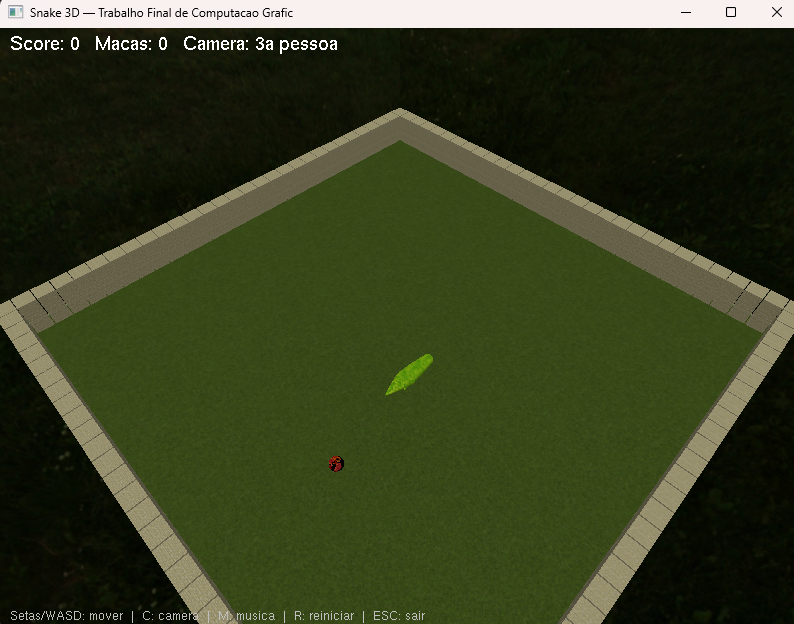
\includegraphics[width=.65\textwidth]{screenshots/jogo-3a-pessoa.png}
\caption{Câmera em terceira pessoa: cobra com corpo afinado, maçã 3D flutuante
         e \textit{skybox}. A borda sólida do mapa é visível ao redor do
         \textit{grid}.}
\label{fig:terceira}
\end{figure}

\begin{figure}[H]
\centering
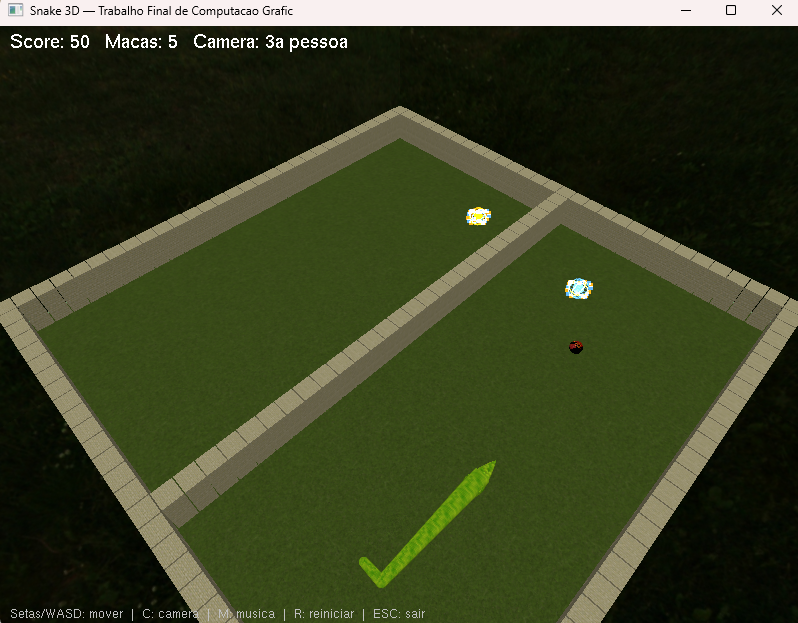
\includegraphics[width=.65\textwidth]{screenshots/parede-portais.png}
\caption{Parede central (textura de \textit{paving stones}) com os dois portais
         animados em evidência. Portal A (laranja) e Portal B (azul) ocupam
         lados opostos da parede.}
\label{fig:parede}
\end{figure}

\begin{figure}[H]
\centering
\includegraphics[width=.65\textwidth]{screenshots/primeira-pessoa.png}
\caption{Câmera em primeira pessoa: visão da perspectiva da cabeça da cobra,
         evidenciando o sombreamento de Gouraud no chão e nas paredes.}
\label{fig:primeira}
\end{figure}

% =============================================================================
\section{Conclusão}

O Snake 3D demonstrou a integração prática dos pilares de Computação Gráfica em uma aplicação interativa. Os principais desafios foram: (1) \textbf{loader OBJ próprio} com suporte aos quatro formatos de face e normalização por \textit{bounding box}; (2) \textbf{orientação dos cilindros} via \texttt{atan2} + \texttt{glRotatef} em Y; (3) \textbf{atlas da maçã sem mipmap} — fundo preto vazava para as bordas, resolvido com \texttt{GL\_LINEAR} sem mipmap; (4) \textbf{normais invertidas} em modelos OBJ eliminadas com \texttt{GL\_LIGHT\_MODEL\_TWO\_SIDE}; (5) \textbf{BGM multiplataforma} (\texttt{mciSendStringA} no Windows vs.\ \texttt{fork}+\texttt{afplay} no macOS).

Como trabalhos futuros destacam-se: \textit{shaders} GLSL (Phong, \textit{normal mapping}, sombras), múltiplas fases, \textit{high score} persistente e IA.

% =============================================================================
\bibliographystyle{sbc}
\bibliography{relatorio}

\end{document}
